% !TEX TS-program = lualatex
%\documentclass[handout]{beamer}
\documentclass{beamer}
\input{../common/misomva}
\begin{document}
% Topic-specific title slide
\newcommand{\topictitle}{Google PageRank: Core Algorithm}
\newcommand{\topicsubtitle}{Steady State and Perron's Theorem}
\newcommand{\misoclasstinytitleslide}{Partially based on material by:  Andreas Krause, \\[-1em] Branislav Kveton, Michael Kearns}

\MakeTopicSlide

\begin{frame}
\frametitle{Success story \#2 \emphcol{Google \pagerank}}
\textbf{Google matrix:} $\bG = (1-p) \bM + p\cdot\tfrac{1}{\nodes} \1_{\nodes \times \nodes}$, where $p=0.15$ \\
\smallskip
\onslide<2-| handout:2->{%
$\bG$ is \textbf{stochastic} \questionbox{why?}   \notecol{\tiny What is $\bG\ba$ for any $\ba$?}
We look for $\bG\bv = 1\times \bv$, steady-state vector, a right eigenvector with eigenvalue 1. 
 \questionbox{why?} 
\\
}
\onslide<3-| handout:2->{%
\smallskip
\textbf{Perron's theorem:} Such $v$ exists and it is \textbf{unique} \\  \quad  if the entries of $\bG$ are positive.
}
\onslide<3-|handout:2->{
\begin{center}
% Manual layout for PageRank graph (spring layout needs lualatex)
\begin{tikzpicture}[font={\tiny\bfseries},
  nd/.style={circle, draw, minimum size=6mm, inner sep=0pt},
  lbl/.style={font=\tiny\bfseries, text=mvaAccent, above=-1pt},
  ->, >=stealth]
\node[nd] (G) at (0,1.5) {\only<3-4| handout:2-3>{\phantom{?}}\only<5-| handout:4>{0.15}};
\node[nd] (A) at (1.5,2.5) {\only<3| handout:2>{?}\only<4| handout:3>{0.15}\only<5-| handout:4>{0.21}};
\node[nd] (B) at (3,1.5) {\only<3| handout:2>{?}\only<4| handout:3>{0.31}\only<5-| handout:4>{0.40}};
\node[nd] (C) at (1.5,0) {\only<3| handout:2>{?}\only<4| handout:3>{0.54}\only<5-| handout:4>{0.67}};
\node[nd] (D) at (3,-1) {\only<3| handout:2>{?}\only<4| handout:3>{0.38}\only<5-| handout:4>{0.44}};
\node[nd] (E) at (0,-1) {\only<3| handout:2>{?}\only<4| handout:3>{0.38}\only<5-| handout:4>{0.44}};
\node[nd] (F) at (1.5,-2.2) {\only<3| handout:2>{?}\only<4| handout:3>{0.64}\only<5-| handout:4>{0.70}};
\only<5-| handout:4>{\draw (G) -> (A); \draw (G) -> (B);}
\draw (A) -> (C);
\draw (B) -> (C);
\draw (C) -> (D);
\draw (D) -> (B);
\draw (D) -> (F);
\draw (C) -> (E);
\draw (E) -> (F);
\end{tikzpicture}
}
 
\end{center}
\end{frame}
%%%%%%%%%%%%%%%%%%%%%%%%%%%%%%%%%%%%%%%%%%%%%%%%%%%%%%%%%


\MakeLastSlide
\end{document}
